% Moves of N_k as rook placements on an n x n board (n = 8).
% Rows = positions t, columns = jobs' new positions sigma(t); shaded = band |t - s| <= k-1.
\documentclass[tikz,border=2pt]{standalone}
\usepackage{amsmath}
\begin{document}
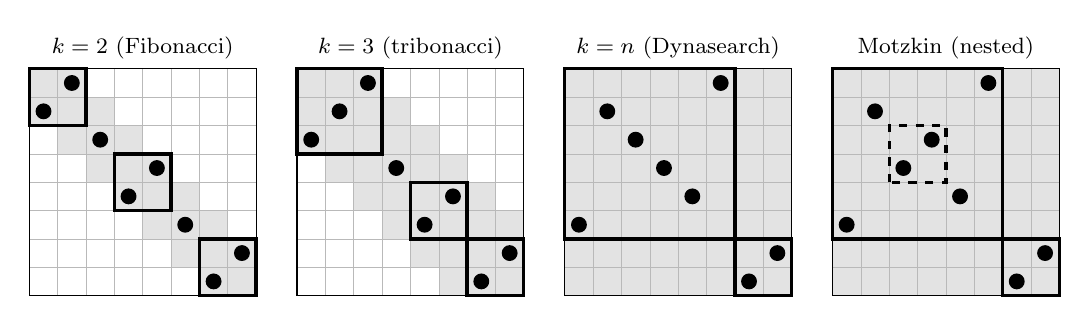
\begin{tikzpicture}[x=0.36cm,y=0.36cm,font=\footnotesize]
% \board{x-offset}{band width k-1}{sigma(1..8)}{title}
\newcommand{\board}[4]{%
  \begin{scope}[xshift=#1 cm]
    \foreach \r in {1,...,8}{\foreach \c in {1,...,8}{%
      \pgfmathtruncatemacro{\dd}{abs(\r-\c)}%
      \ifnum\dd<\numexpr#2+1\relax
        \fill[gray!22] (\c-1,-\r) rectangle (\c,-\r+1);
      \fi}}
    \foreach \i in {1,...,7}{\draw[gray!55,very thin] (\i,-8) -- (\i,0); \draw[gray!55,very thin] (0,-\i) -- (8,-\i);}
    \draw (0,-8) rectangle (8,0);
    \foreach [count=\r] \c in {#3}{\fill (\c-0.5,-\r+0.5) circle (0.28);}
    \node[above] at (4,0) {#4};
  \end{scope}}
% block outline on the diagonal: \blk{x-offset}{first}{last}
\newcommand{\blk}[3]{\draw[very thick,xshift=#1 cm] (#2-1,-#3) rectangle (#3,-#2+1);}

\board{0}{1}{2,1,3,5,4,6,8,7}{$k=2$ (Fibonacci)}
\blk{0}{1}{2}\blk{0}{4}{5}\blk{0}{7}{8}

\board{3.4}{2}{3,2,1,4,6,5,8,7}{$k=3$ (tribonacci)}
\blk{3.4}{1}{3}\blk{3.4}{5}{6}\blk{3.4}{7}{8}

\board{6.8}{7}{6,2,3,4,5,1,8,7}{$k=n$ (Dynasearch)}
\blk{6.8}{1}{6}\blk{6.8}{7}{8}

\board{10.2}{7}{6,2,4,3,5,1,8,7}{Motzkin (nested)}
\blk{10.2}{1}{6}\blk{10.2}{7}{8}
\draw[very thick,dashed,xshift=10.2cm] (2,-4) rectangle (4,-2);
\end{tikzpicture}
\end{document}
